\documentclass{uvamscse}

% \usepackage{listings}
% \usepackage{boxedminipage}
% \usepackage{multicol}
% \usepackage[Symbol]{upgreek}
% \usepackage{tikz}
% \usepackage{xspace}
% \usepackage{amssymb}
% \usepackage{amsmath}

\newcommand{\cmd}[1]{\texttt{$\backslash$#1}}

\title{MetaThesis}
% \coverpic[100pt]{figures/terminal.png}
\subtitle{A Thesis Template Leading by Example}
% \date{Spring 2014}

\author{Vadim Zaytsev}
\authemail{vadim@grammarware.net}
% \host{FacePalmBeach, \url{http://grammarware.github.io}}

\abstract{
  This section summarises the content of the thesis for potential readers who do not have time to read it whole,
  or for those undecided whether to read it at all. Sum up the following aspects:

  \begin{itemize}
    \item relevance and motivation for the research
    \item research question(s) and a brief description of the research method
    \item results, contributions and conclusions
  \end{itemize}
}


\begin{document}
\maketitle

%%%%%%%%%%%%%%%%%%%%%%%%%%%%%%%%%%%%%%%%%%%%%%%%%%%%%%%%%%%%%%%%%%%%%%%%%%%%%%%%
\chapter{Front Matter}

\section{Title}

Specify the title of the thesis with \cmd{title} and \cmd{subtitle} commands:

\begin{snippet}
\begin{verbatim}
\title{MetaThesis}
\subtitle{A Thesis Template Leading by Example}
\end{verbatim}
\end{snippet}

Any thesis can survive without a \cmd{subtitle}, but the \cmd{title} is mandatory.

\section{Author}

Introduce yourself with \cmd{author} and \cmd{authemail}:

\begin{snippet}
\begin{verbatim}
\author{Vadim Zaytsev}
\authemail{vadim@grammarware.net}
\end{verbatim}
\end{snippet}

Again, \cmd{authemail} is not mandatory. If you need anything fancier, just put it inside \cmd{author}.

\begin{snippet}
\begin{verbatim}
\author{Vadim Zaytsev\footnote{Yes, that one.}}
\end{verbatim}
\end{snippet}

The footnote would be printed on the bottom of the title page, and will be
referred to by a symbol, not by a number as any footnotes within the main
document body.

\section{Date}

By default, the date inserted in your PDF is the day of the build, e.g., ``March 25, 2014''. If you want it to be formatted differently or be more vague or outright fake, use \cmd{date}:

\begin{snippet}
\begin{verbatim}
\date{Spring 2014}
\end{verbatim}
\end{snippet}

or even

\begin{snippet}
\begin{verbatim}
\date{Tomorrow. Honestly.}
\end{verbatim}
\end{snippet}

\section{Host}

If your hosting organisation is not the UvA, specify it with \cmd{host}. The
logo on the bottom of the title page will still be the UvA one, because this
is the organisation guaranteeing your degree.

\begin{snippet}
\begin{verbatim}
\host{FacePalmBeach, \url{http://grammarware.github.io}}
\end{verbatim}
\end{snippet}

NB: footnotes will not work, unless you know how to \cmd{protect} them.

\section{Cover picture}

If the first page of your thesis looks too blunt, add a picture to it:

\begin{snippet}
\begin{verbatim}
\coverpic{figures/terminal.png}
\end{verbatim}
\end{snippet}

You can even specify the picture's width as an optional argument:

\begin{snippet}
\begin{verbatim}
\coverpic[100pt]{figures/terminal.png}
\end{verbatim}
\end{snippet}

How these three options look, you can see from \autoref{fig:titles}.

\begin{figure}[t]
  \fbox{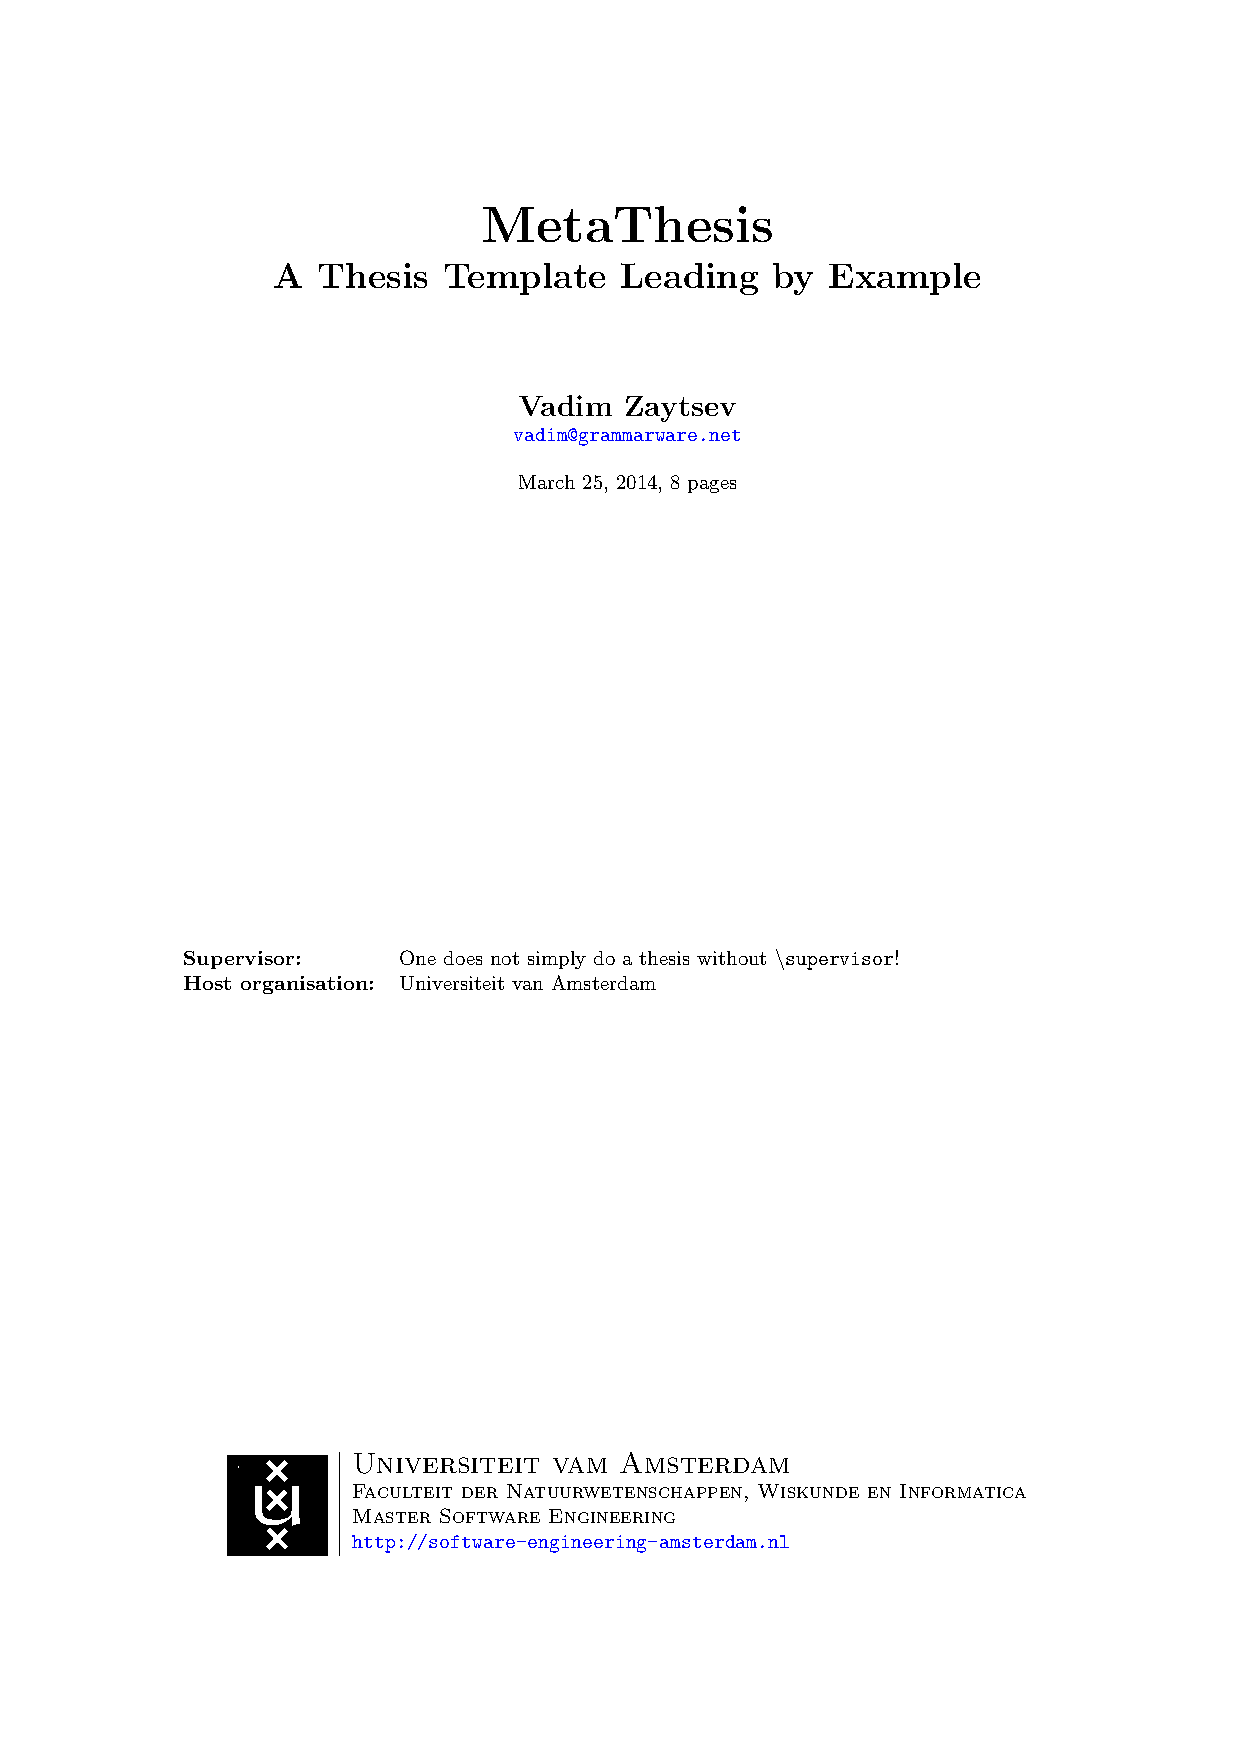
\includegraphics[width=.25\textwidth]{figures/title1.pdf}}
  \hfill
  \fbox{
\includegraphics[width=.25\textwidth]{figures/title2.pdf}}
  \hfill
  \fbox{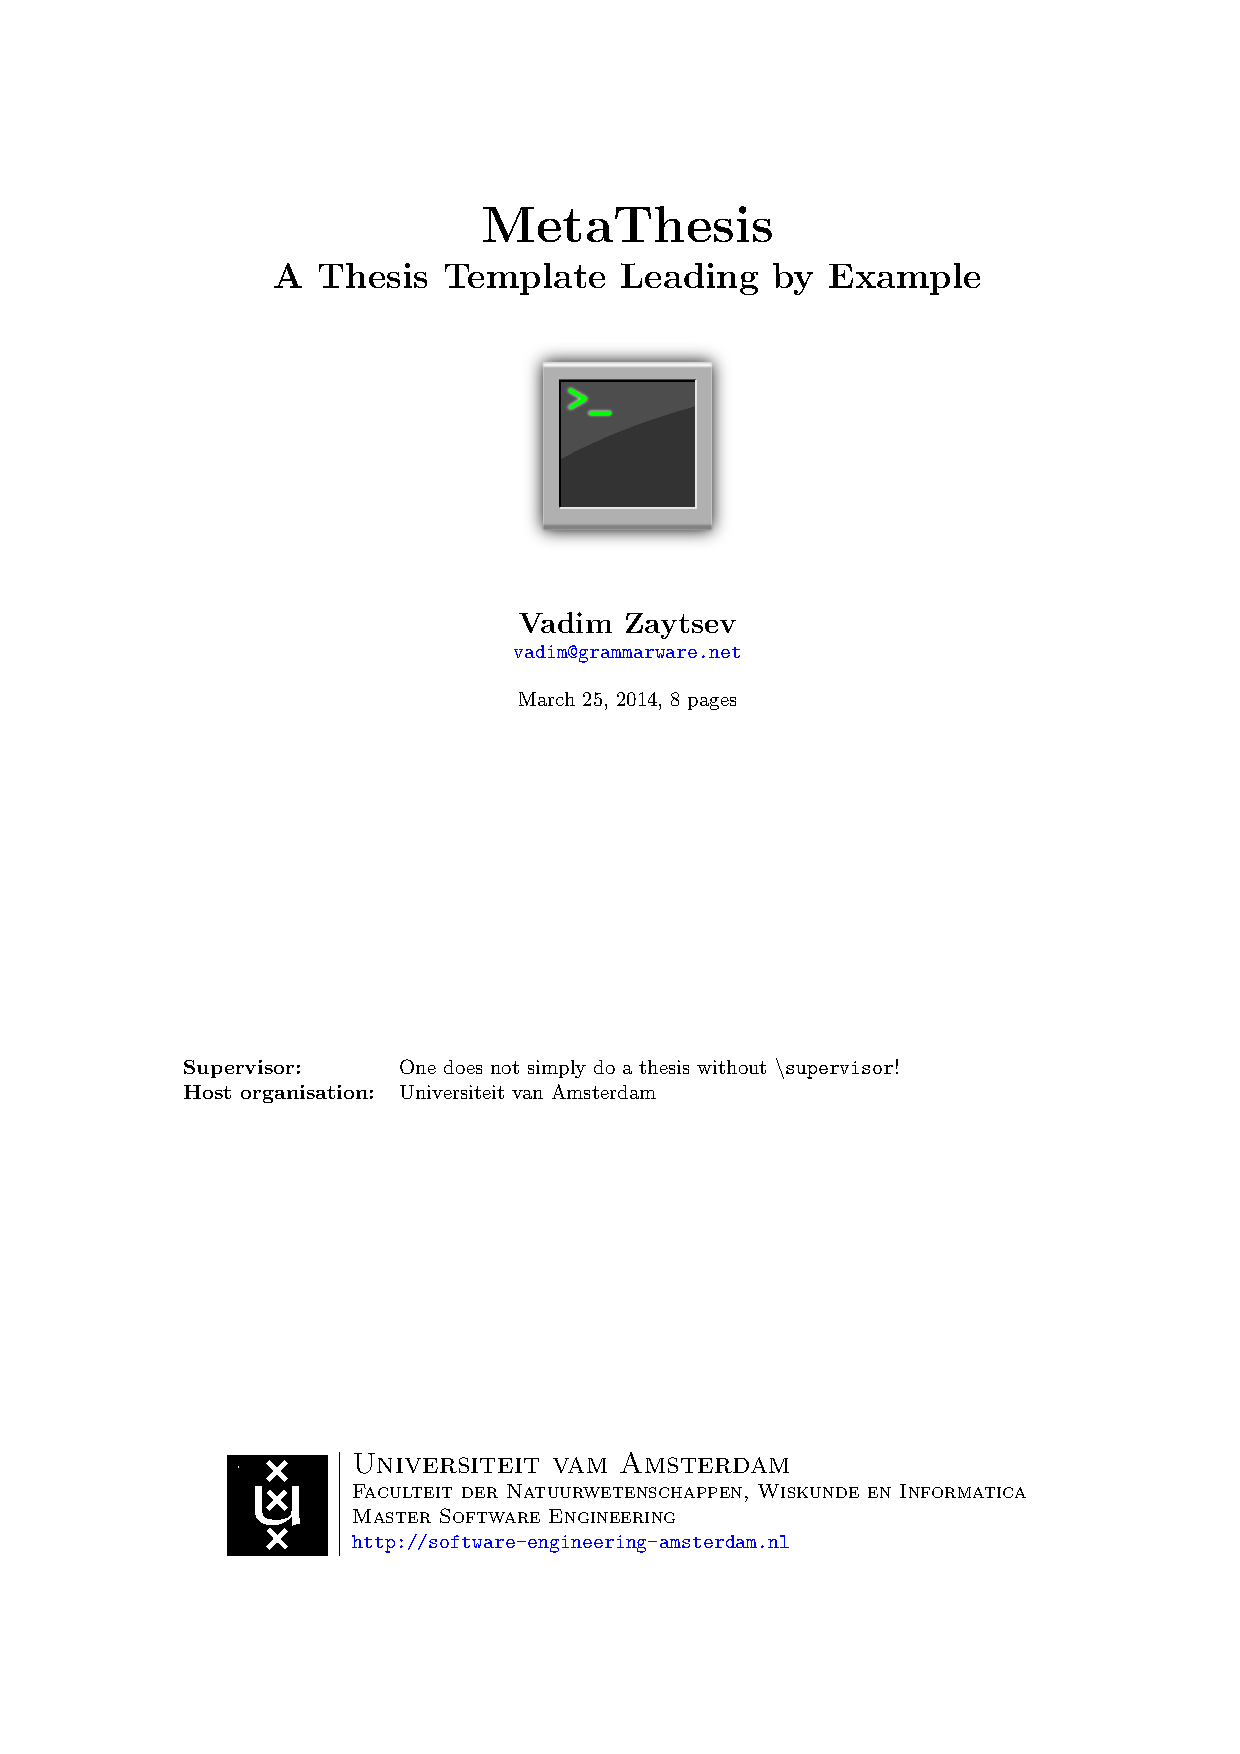
\includegraphics[width=.25\textwidth]{figures/title3.pdf}}
  \caption{A hypothetical thesis title page without a cover picture (on the left), with an overly large one (in the cenre) and with a tiny pic (on the right).}
  \label{fig:titles}
\end{figure}

\section{Abstract}

A thesis is fine without an abstract, if you do not feel like writing it and
your supervisor does not feel like enforcing it. If you do want an abstract,
make it with the \cmd{abstract} command:

\begin{snippet}
\begin{verbatim}
\abstract{This is not a thesis.}
\end{verbatim}
\end{snippet}

The abstract is just like any other section of your thesis, so you can use any
\LaTeX\ tricks there. If you think that the name ``abstract'' is too abstract
for your abstract, you can still use \cmd{abstract} without being too
abstract:

\begin{snippet}
\begin{verbatim}
\abstract[Confession]{I am a cenosillicaphobiac.}
\end{verbatim}
\end{snippet}

Kent Beck~\cite{JohnsonBBCGW93} proposes to have four sentences in a good abstract:

\begin{enumerate}
  \item The first states the problem.
  \item The second states why the problem is a problem.
  \item The third is the startling sentence.
  \item The fourth states the implication of the startling sentence.
\end{enumerate}

In practice, each of these ``sentences'' can be longer than an actual
sentence, but it is in general a good rule of thumb to condense the summary of
your thesis into these four tiny messages. Do not write too much, make it
tweetable.

%%%%%%%%%%%%%%%%%%%%%%%%%%%%%%%%%%%%%%%%%%%%%%%%%%%%%%%%%%%%%%%%%%%%%%%%%%%%%%%
\chapter{Core Chapters}

The structure of your thesis is up to you and your supervisor. Whatever you
do, do not consider the guidelines below as dogmas.

\section{Classic structure}

\begin{description}
  \item[Problem statement and motivation.]
  You describe in detail what problem the research is addressing, and what is
the motivation to address this problem. There is a concise and objective
statement of the research questions, hypotheses and goals. It is made clear
why these questions and goals are important and relevant to the world outside
the university (assuming it exists). You can already split the main research
question into subquestions in this chapter. This section also describes an
analysis of the problem: where does it occur and how, how often, and what are
the consequences? An important part is also to scope the research: what
aspects are included and what aspects are deliberately left out, and why?
  \item[Research method.]
  Here you describe the methods used to answer the research questions. A good
structure of this section often follows the subquestions by providing a method
for each. The research method needs a thorough motivation grounded in theory
in order to be acceptable. As a part of the method, you can introduce a number
of hypotheses --- these will be tested by the research, using the methods
described here. An important part of this section is validation. How will you
evaluate and validate the outcomes of the research?
  \item[Background and context.]
  This chapter contains all the information needed to put the thesis into
context. It is common to use a revised version of your literature survey for
this purpose. It is important to explicitly refer from your text to sources
you have used, they will be listed in your bibliography. For example, you can
write ``A small number of programming languages account for most language
use~\cite{MeyerovichR2013}'', where the following entry would be included in
your bibliography:
\begin{quote}
\cite{MeyerovichR2013} Leo A. Meyerovich and Ariel S. Rabkin. Empirical Analysis of Programming Language Adoption. In \emph{Proceedings of the 2013 ACM SIGPLAN International Conference on Object Oriented Programming Systems Languages and Applications}, OOPSLA, pages 1--18. ACM, 2013. \doi{10.1145/2509136.2509515}.
\end{quote}
Have a look at \autoref{sec:biblio} to learn more about citation.
  \item[Research.]
  This chapter reports on the execution of the research method as described in
an earlier chapter. If the research has been divided into phases, they are
introduced, reported on and concluded individually. If needed, this chapter
could be split up to balance out the sizes of all chapters.
  \item[Results.]
  This chapter presents and clarifies the results obtained during the
  research. The focus should be on the factual results, not the interpretation
  or discussion. Tables and graphics should be used to increase the clarity of
  the results where applicable.
  \item[Analysis and conclusions.]
  This chapter contains the analysis and interpretation of the results. The
  research questions are answered as best as possible with the results that
  were obtained. The analysis also discussed parts of the questions that were
  left unanswered.

  An important topic is the validity of the results. What methods of
  validation were used? Could the results be generalised to other cases? What
  threats to validity can be identified? There is room here to discuss the
  results of related scientific literature here as well. How do the results
  obtained here relate to other work, and what consequences are there? Did
  your approach work better or worse? Did you learn anything new compared to
  the already existing body of knowledge? Finally, what could you say in
  hindsight on the research approach by followed? What could have done better?
  What lessons have been learned? What could other researchers use from your
  experience? A separate section should be devoted to ``future work'', i.e.,
  possible extension points of your work that you have identified. Even other
  researchers should be able to use those as a starting point.
\end{description}

\section{Reporting on replications}

Here are the guidelines to report on replicated studies~\cite{Carver10}:

\begin{description}
  \item[Information about the original study]~\\
    \begin{description}
    \item[Research question(s)] that were the basis for the design
    \item[Participants,] their number and any other relevant characteristics
    \item[Design] as a graphical or textual description of the experimental design
    \item[Artefacts,] the description of them and/or links to the artefacts used
    \item[Context variables] as any important details that affected the design of the study or interpretation of the 
results
    \item[Summary of the results] in a brief overview of the major findings
    \end{description}
  %
  \item[Information about the replication]~\\
    \begin{description}
    \item[Motivation for conducting the replication] as a 
description of why the replication was conducted: 
to validate the results, to broaden the results by 
changing the participant pool or the artifacts. 
    \item[Level of interaction with original experimenters.]
The level of interaction between the original experimenters and the
replicators should be reported. This interaction could range from none (i.e.
simply read the  paper) to them being the same people. There is quite a lot of
discussion of the level of interaction allowed for the replication to be
``successful'', but this level should be reported even without  addressing
the controversy.
    \item[Changes to the original experiment.] Any changes made to the
design, participants, artifacts, procedures, data collected and/or analysis
techniques should be  discussed along with the motivation for the change.
    \end{description}
  \item[Comparison of results to original]~\\
    \begin{description}
    \item[Consistent results,] when replication results supported 
results from the original study, and 
    \item[Differences in results,] when results from the replication 
did not coincide with the results from the original study. 
Authors should also discuss how changes made to the 
experimental design (see above) may have caused 
these differences. 
    \end{description}
    \item[Drawing conclusions across studies]
\end{description}

NB: this section contains portions of text repeated directly from Carver~\cite{Carver10}.
    Do not do this for your thesis.

{%\tiny
\bibliographystyle{alphaurl}
\bibliography{thesis}
}

\end{document}
